\documentclass[../main.tex]{subfiles}
\graphicspath{{\subfix{../../images/}}}

\begin{document}

Sending data across large distances is used all the time, like in video chats, voice chats, uploading homework or simply loading HTML\footnote{This markup language, commonly mistaken for a programming language is what lays out websites; it dictates the structure of the site, like the bricks for a house.}. Typically, sending data like this is done through a stream of \textbf{data packets}, otherwise known as just packets.

A packet looks like the following:

\begin{figure}[h]
    \centering
    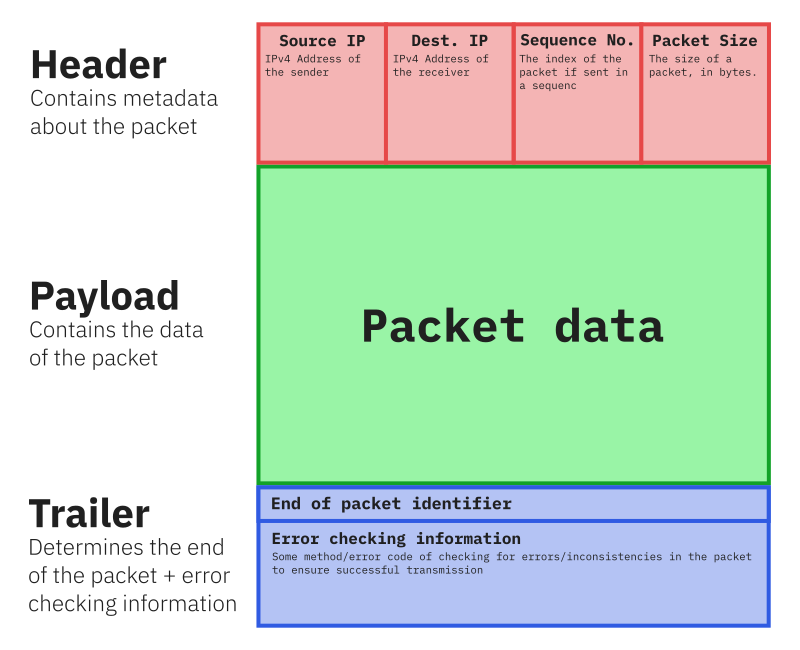
\includegraphics[width=0.6\textwidth]{packet.png}
    \caption{The components of a data packet.}
    \label{fig:packet}
\end{figure}

\subsection{Components of a packet}

\paragraph{The Header}

Contains metadata\footnote{Supporting information, like clarifications in non-fictional texts.} about the packet (see figure \ref{fig:packet}):

\begin{itemize}
    \item The IP\footnote{IP Address; in this context, always IPv4 unless if specified} of the sender
    \item The IP of the receiver
    \item The sequence number; If a lot of data must be sent throughout multiple packets, the
          \emph{sequence number} makes sure that the packets' payloads are reassembled in the correct order.
    \item The packet size, in order to make sure the packet received is of the correct size.
\end{itemize}

\paragraph{The Payload}

Consists of the binary data to be transmitted via the packet (see figure \ref{fig:packet}).

\paragraph{The Trailer}

Consists of the following (see figure \ref{fig:packet}):

\begin{itemize}
    \item Some way of identifying the end of the packet. This is typically some special value like a null terminator\footnote{In programming,
          this is referred to as a \emph{sentinel value}, which just means a value that carries some special meaning. An example is like in the
          C programming language, to tell the end of a string, a sentinel value of 0 is used to denote the string finished.}. The algorithm can
          then scan the data until it hit that character to extract the payload.
    \item An error checking method. CRCs are used to check this.
\end{itemize}

\paragraph{Packet Switching}

In order to transfer packets from one place to another

\end{document}
